\newsavebox{\fmbox}
\newenvironment{fmpage}[1]
     {\begin{lrbox}{\fmbox}\begin{minipage}{#1}}
     {\end{minipage}\end{lrbox}\fbox{\usebox{\fmbox}}}

\chapter{Réalisation}

Sous \imj, il existe deux types de plugins : \emph{PlugInFilter} et \emph{PlugInFrame}. Étant donné que nous avions besoin de différents objets graphiques, nous avons choisi d'utiliser \emph{PlugInFrame}. C'est la classe \texttt{Pick\_EM} qui en hérite et permet de lancer notre plugin à son appel par l'intermédiaire de la barre de menus d'\imj.

\section{Interface graphique}

\subsection{Panneaux et boutons}

Nos panneaux dérivent de la classe \emph{JPanel}, elle-même issue de la classe \emph{Panel}. Cette dernière fournit un composant Container permettant d'accueillir d'autres composants graphiques (sous-panneaux).\\

Le premier panneau (\textbf{panel1}) contient une zone de texte (\emph{JLabel}) afin d'afficher un message d'aide, ainsi qu'un menu déroulant (\emph{JComboBox}) pour le choix des algorithmes. \\

Le panneau central (\textbf{panel2}) est vide au lancement du plugin et son contenu varie en fonction de l'algorithme sélectionné. Par exemple pour l'algorithme Difference of Gaussian, les sous-panneaux sont créés dans la classe \texttt{panelDoG}. Pour cet algorithme, le \textbf{panel2} comprend :
\begin{itemize}
\item \textbf{infoPanel} contenant un \emph{JLabel} indiquant le type d'image requis.
\item \textbf{sigmaPanel} et \textbf{widthNoisePanel} qui contiennent des \emph{JLabel} et \emph{JTextField} afin de créer une zone dans laquelle peut entrer les paramètres nécessaires au déroulement du piquage. 
\item \textbf{debugCropPanel} quand à lui contient deux cases à cocher (\emph{JCheckBox}) pour activer ou non les modes de débogage et de crop. 
\end{itemize}
Les classes \texttt{panelImCorr} et \texttt{panelDilateDiff} servent à la création des sous panneaux des algorithmes Image Correlation et Dilate Difference respectivement. \\

Le dernier panneau (\textbf{panel3}) comporte quatre boutons (\emph{JButton}) devant répondre aux clics de la souris à l'aide d'un \emph{ActionListener}. \\

Enfin, le panneau principal (\textbf{mainPanel}) contient tous les panels cités précédemment. Sa taille détermine celle de la fenêtre du plugin. \\
Ces quatre panneaux sont crées dans la classe \texttt{PickFrame}, qui hérite de la classe \texttt{JFrame}. \texttt{PickFrame} peut également accéder à des méthodes de la classe \texttt{ActionListener}. \\

La figure suivante (Figure \ref{panneauxDetail}) donne un aperçu plus visuel de l'organisation de ces différents panneaux.
\begin{figure}[!ht] 
\begin{center}
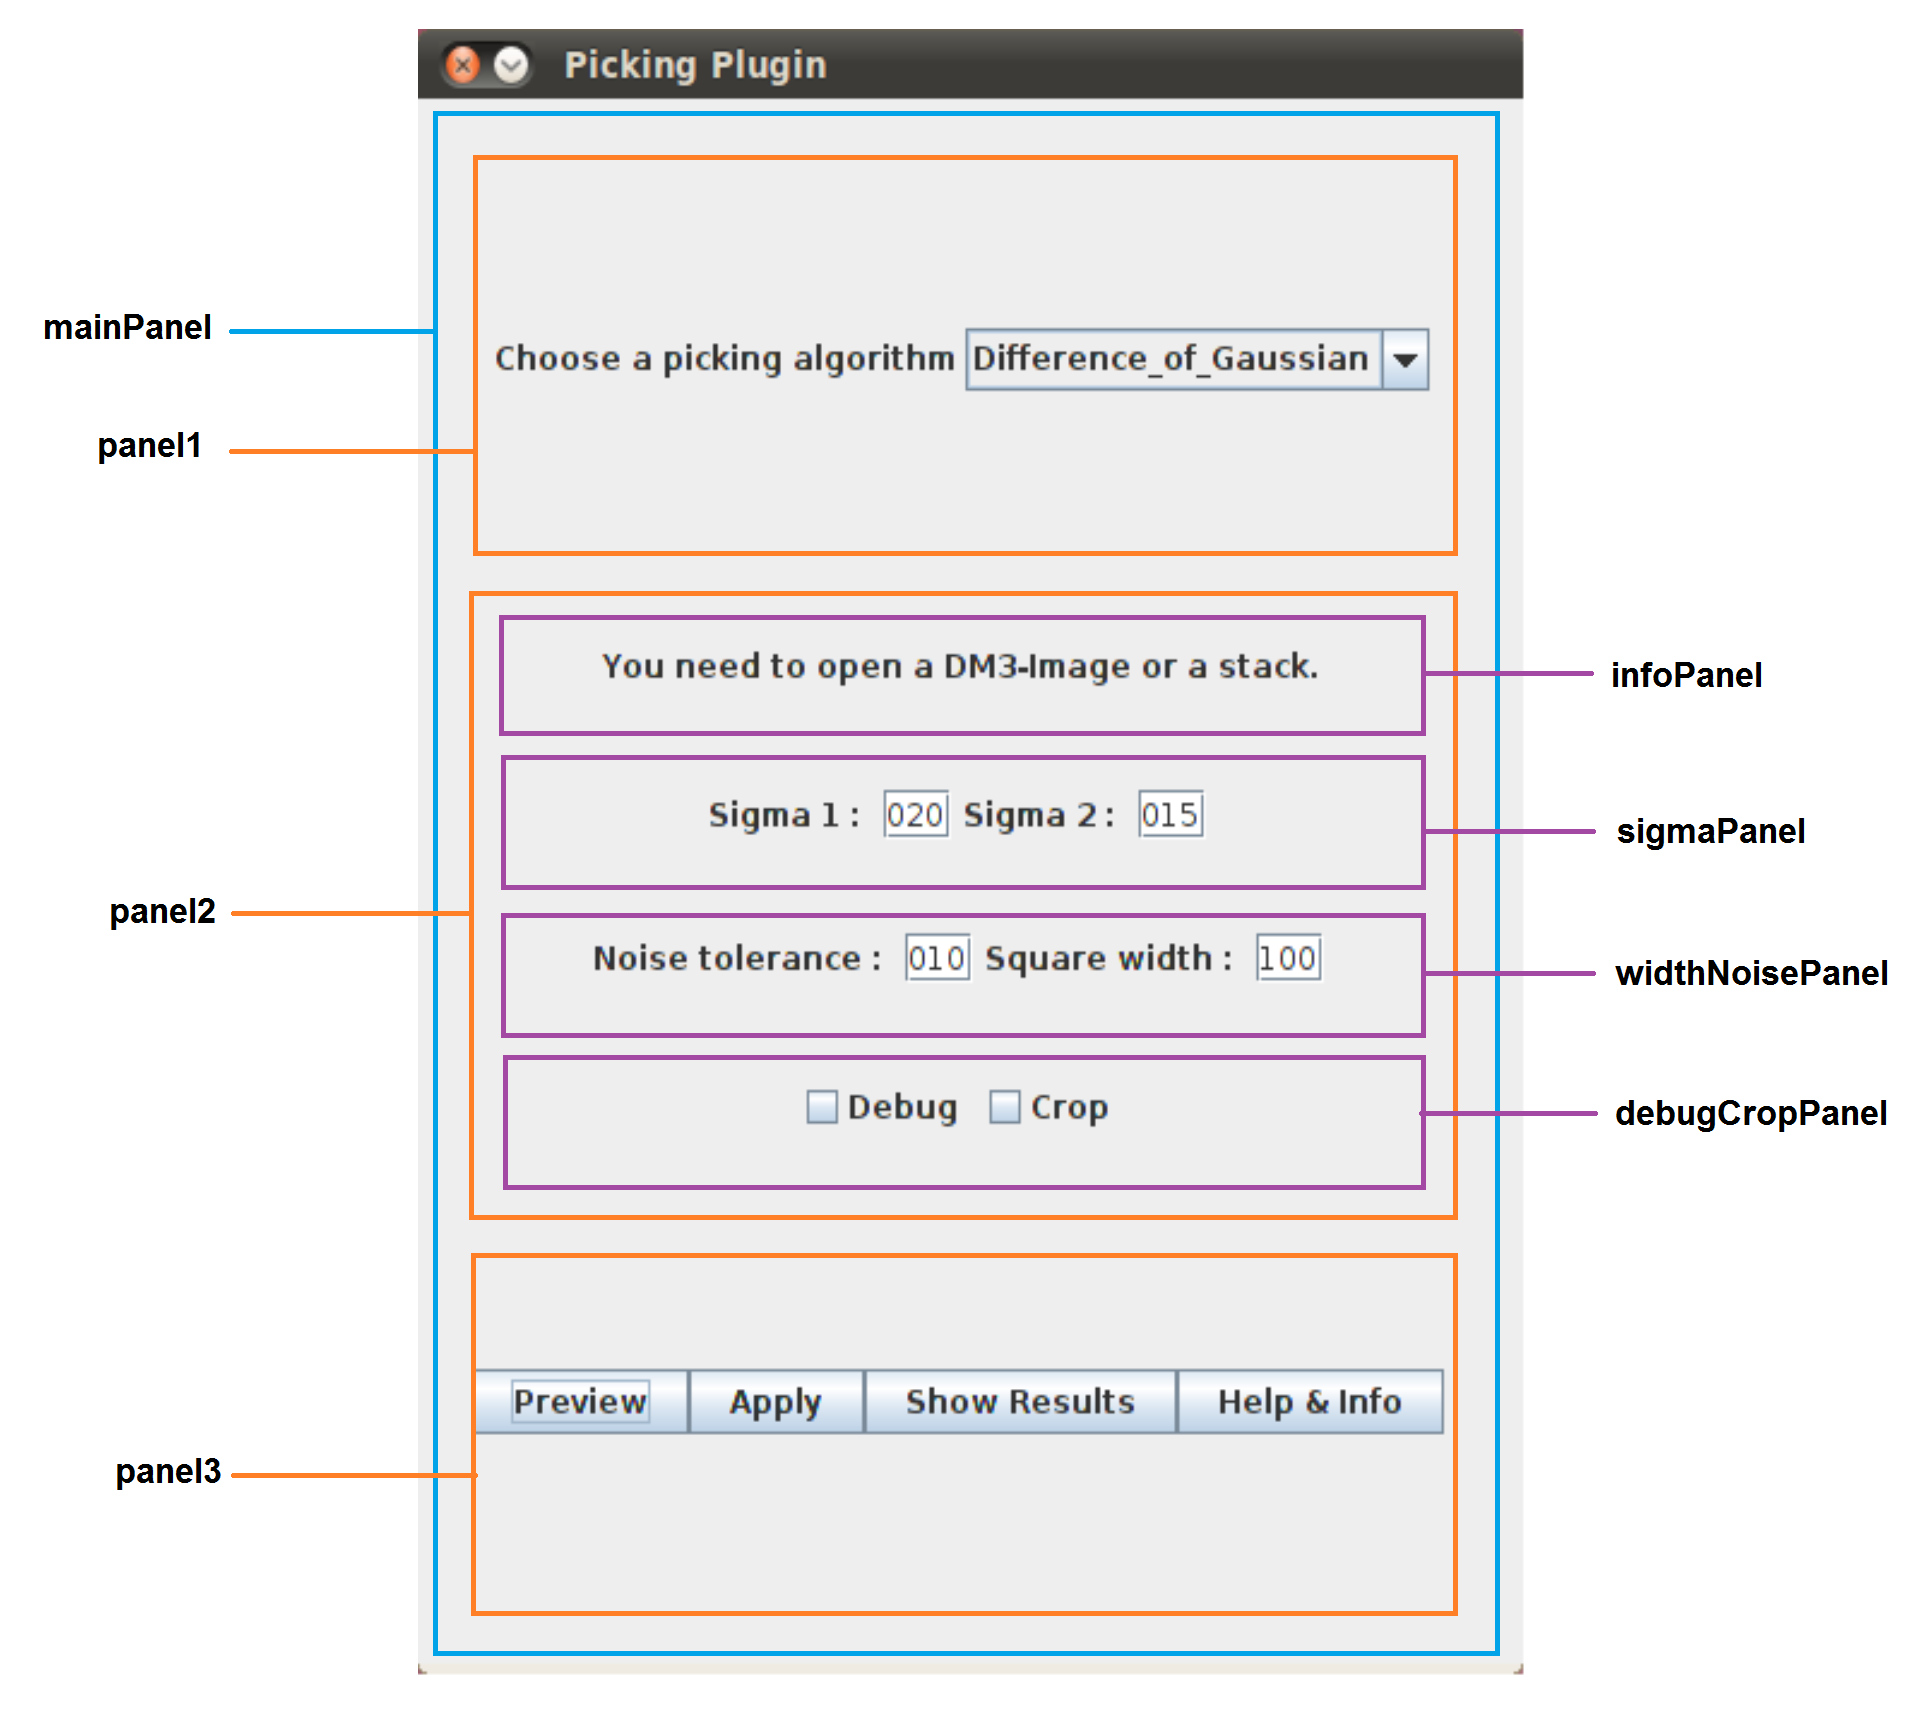
\includegraphics[width=0.8\textwidth]{plugin3-1.png}
\caption{Organisation des panels pour l'algorithme Difference of Gaussian}
\label{panneauxDetail}
\end{center}
\end{figure}
\pagebreak

La classe \texttt{PickFrame} permet donc de générer l'interface graphique du plugin. De plus, elle permet de réagir lors d'un clic sur un bouton. C'est la méthode \texttt{actionPerformed()} qui vérifie le nom de l'algorithme choisi par l'utilisateur parmi ceux proposés dans la JComboBox et permet d'afficher le panel2 qu'il faut. Ci-après un extrait de la méthode \texttt{actionPerformed()} :

\begin{center}
\begin{fmpage}{15cm}
\begin{small}
\begin{lstlisting}[breaklines=true, breakatwhitespace=true]
public void actionPerformed(ActionEvent e) {
  String command = e.getActionCommand();
  String comboSelection = null;
  if (command.equals("comboBoxChanged")){
    JComboBox cb = (JComboBox)e.getSource();
    comboSelection = (String) cb.getSelectedItem();
    panel2.removeAll();
    // Allows the panel2's update
    mainPanel.remove(panel1);
    mainPanel.remove(panel2);
    mainPanel.remove(panel3);
    panel2 = AlgoFactory.algorithm.getPickPanel(comboSelection);
    mainPanel.add(panel1);
    mainPanel.add(panel2);
    mainPanel.add(panel3);
    mainPanel.repaint();
    pack();
  }
\end{lstlisting}
\end{small}
\end{fmpage}
\end{center}

Comme nous avions quelques soucis d'actualisation des panneaux, lors de l'implémentation, nous avons décidé de les supprimer puis de les recréer lors de chaque changement d'algorithme. Le chargement du bon panel2 se fait gr\^ace à \texttt{getPickPanel} de la classe \texttt{AlgoFactory}. \texttt{pack()} permet de recadrer la fenêtre en fonction de son contenu. 

\begin{center}
\begin{fmpage}{15cm}
\begin{small}
\begin{lstlisting}
if (command.equals("Apply")){
  comboSelection = (String)algoList.getSelectedItem();
  Attributes.getInstance();
  coordXYZ = AlgoFactory.algorithm.getPicker(comboSelection);
  IJ.showStatus("End of picking");
}
else if (command.equals("Preview")){
  comboSelection = (String)algoList.getSelectedItem();
  Attributes.getInstance();
  AlgoFactory.algorithm.getPickerPreview(comboSelection);
  IJ.showStatus("End of Preview");
}
else if (command.equals("Show Results")){
  ToCSV.generateCsvFile(coordXYZ);
}
\end{lstlisting}
\end{small}	
\end{fmpage}
\end{center}

\paragraph*{}
Grâce à cette série structures conditionnelles, il est possible d'appliquer les méthodes de piquage appropriées en fonction du choix de l'utilisateur. Le lancement de la procédure ne se fait que si ce dernier clique sur les boutons de prévisualisation ou d'application. La tableau de résultats ne sera généré que s'il appuie sur le bouton d'affichage des résultats. 

\subsection{Affichage des résultats}

Lorsque l'utilisateur a coché la case "crop" avant de lancer la procédure de piquage, la classe \texttt{PickFrame} fait appel à la classe \texttt{Cropper} permettant de créer un stack. Les paramètres d'entrée de \texttt{Cropper()} sont une \emph{ImagePlus} (image courante du stack) et un tableau de doubles contenant les coordonnées des particules sélectionnées. \\
Lors de nos phases de tests, nous avons ajouté une autre fonction Cropper(), sans paramètres d'entrée. Nous y avons créé un tableau de coordonnées manuellement pour faciliter les essais. \\
A partir du tableau de doubles cité, la méthode \texttt{crop()} de \texttt{Cropper} fait appel à la méthode \texttt{setRoi()} d'\imj ~afin de retenir une zone carrée autour de la sélection. Cette zone va ensuite être dupliquée et ajoutée au stack sous la forme d'un \emph{ImageProcessor}. Ci-dessous un extrait de la méthode \texttt{crop()} : 

\begin{center}
\begin{fmpage}{16cm}
\begin{small}
\begin{lstlisting}
if (z == currentSlice) {
  imp.setRoi(x, y, widthCrop, widthCrop);  
  // widthCrop = taille du carre de selection entree par l'utilisateur
  img2 = new Duplicator().run(imp);
  ImageProcessor ip2 = img2.getProcessor();
  ImageProcessor impTemp = ip2.resize(widthCrop,widthCrop);
  ims.addSlice(impTemp);
}
\end{lstlisting}
\end{small}	
\end{fmpage}
\end{center}

\paragraph*{}
Cette partie du code ne va s'exécuter que si le cadre de sélection de la particule ne dépasse pas le cadre de l'image de base. Les particules dépassant n'apparaitront pas dans le stack d'imagettes, mais on pourra retrouver leurs coordonnées dans le tableau de résultats final. \\

Par ailleurs, les résultats de la sélection peuvent être affichés sous la forme d'une \texttt{ResultsTable} si on clique sur le bouton "Show Results". Elle est construite grâce au tableau de doubles cité précédemment, qui est le paramètre d'entrée de la fonction \texttt{generate-} \texttt{CsvFile()}. 

\section{Récupération des paramètres}

Le singleton de la classe \texttt{Attributes} contient une table de hashage (\emph{HashTable}) dans laquelle sont stockés tous les paramètres entrés par l'utilisateur. Ces derniers sont accessibles grâce à des clés et donc réutilisables dans les algorithmes. La méthode  \texttt{synchronized()} dans la fonction \texttt{getInstance()} (voir ci-dessous) empêche toute instanciation multiple :

\begin{center}
\begin{fmpage}{11cm}
\begin{small}
\begin{lstlisting}
public final static Attributes getInstance() {
  if (Attributes.instance == null) {
    synchronized(Attributes.class) {
      if (Attributes.instance == null) {
        Attributes.instance = new Attributes();
      }
    }
  }
  return Attributes.instance;
}
\end{lstlisting}
\end{small}	
\end{fmpage}
\end{center}

\pagebreak

\section{Algorithmes}

\subsection{Comparaison langage Macro \imj ~et \java}

Nous avons commencé par implémenter les algorithmes grâce à l'outil Macro d'\imj lors de nos  phases de test. Nous les avons ensuite traduits en \java et liés à la partie interface graphique du code. Vous trouverez ci-après un exemple de cette transformation. \\

Extrait de la Macro de la Différence de dilatation :
\begin{center}
\begin{fmpage}{16cm}
\begin{small}
\begin{lstlisting}
run("Blobs (25K)");
run("Duplicate...", "title=blobs-1.gif");
run("Duplicate...", "title=blobs-2.gif");
run("Dilate");
run("Make Binary");
selectWindow("blobs-1.gif");
run("Make Binary");
run("Dilate");
run("Options...", "iterations=2 count=1 edm=Overwrite do=Nothing");
selectWindow("blobs-2.gif");
run("Dilate");
imageCalculator("Subtract create", "blobs-2.gif","blobs-1.gif");
selectWindow("Result of blobs-2.gif");
run("Find Maxima...", "noise=3 output=[Point Selection]");
\end{lstlisting}
\end{small}	
\end{fmpage}
\end{center}

\paragraph*{}
Équivalent en langage \java :
\begin{center}
\begin{fmpage}{16cm}
\begin{small}
\begin{lstlisting}
ImagePlus imp = WindowManager.getCurrentImage();
ImagePlus imp1=new Duplicator().run(imp);
ImagePlus imp2= new Duplicator().run(imp1);
imp1.setSlice(currentslice);
imp2.setSlice(currentslice);
IJ.run(imp1, "Make Binary", "calculate");
IJ.run(imp2, "Make Binary", "calculate");
IJ.run(imp1, "Options...", it1);
IJ.run(imp1, "Dilate", "slice");
IJ.run(imp2, "Options...", it2);
IJ.run(imp2, "Dilate", "slice");
ic = new ImageCalculator();
ImagePlus imp3 = ic.run("Subtract create", imp2, imp1);
ImageProcessor ip3 = imp3.getProcessor();
ip3.invert();
Polygon points = mf.getMaxima(ip3, tolerance, excludeOnEdges);
\end{lstlisting}
\end{small}	
\end{fmpage}
\end{center}

\subsection{Méthodes de piquage}

Lorsque l'utilisateur fait le choix d'un algorithme de piquage parmi ceux qui lui sont proposés, cela fait appel à la classe \texttt{AlgoFactory} contenant plusieurs méthodes switch :
\begin{itemize}
\item \texttt{getPickPanel()} permet de récupérer le nom de l'algorithme choisi et d'afficher le panel2 correspondant.
\item \texttt{getPicker()} permet de lancer le piquage lorsque l'utilisateur appuie sur le bouton Apply.
\item \texttt{getPickerPreview()} permet de lancer le piquage lorsque l'utilisateur appuie sur le bouton Preview.
\end{itemize}

La présence d'un constructeur privé dans cette classe supprime le constructeur public par défaut. De plus, seul le singleton peut s'instancier lui même. \\

Une fois le panel2 chargé, l'appel aux procédures de piquage ne peut se faire que si l'on clique sur les boutons de prévisualisation (Preview) ou d'application à l'ensemble du stack (Apply). \\
Les paramètres entrés par l'utilisateur sont sauvegardés dans la table de hashage grâce à la fonction \texttt{getInstance()} de la classe \texttt{Attributes}. Dans le cas où l'utilisateur entrerait des valeurs non numériques, c'est \imj ~qui se chargerait de gérer les erreurs. \\
Les paramètres sont ensuite récupérés, pour l'algorithme, par la fonction \texttt{setAttributes()} de la classe \texttt{PanelDoG} (pour suivre notre scénario). \\
 L'algorithme est par la suite appelé par la méthode \texttt{sliceSelection()} (Apply) ou par \texttt{picking()} (Preview). \\

La méthode \texttt{picking()} donne l'image courante du stack en paramètre de la méthode \texttt{pick()} alors que \texttt{sliceSelection()} parcourt le stack et appelle \texttt{pick()} autant de fois qu'il y a d'images dans le stack. \\

La méthode \texttt{pick()} quand à elle permet de lancer l'algorithme sur la sélection. Elle prend une ImagePlus et le numéro de l'image dans le stack en paramètres. Cette fonction récupère les paramètres entrés par l'utilisateur (grâce à \texttt{hashAttributes.get()}) et renvoie un tableau de résultats (X, Y, Slice). Voici un extrait du code de l'algorithme Difference of Gaussian :

\begin{center}
\begin{fmpage}{16cm}
\begin{small}
\begin{lstlisting}
Hashtable<String, String> hashAttributes = Attributes.getAttributes();
String sigma1 = hashAttributes.get("sig1");

imp.setSlice(currentslice);
ImagePlus imp1 = new Duplicator().run(imp);

String si1 = "sigma=" + sigma1;

imp1.setSlice(currentslice);
IJ.run(imp1, "Gaussian Blur...", si1);
\end{lstlisting}
\end{small}
\end{fmpage}
\end{center}

Ici, nous obtenons le paramètre \textbf{sigma1} grâce à la table de hashage et la clé "\texttt{sig1}". Nous avons besoin de ce dernier pour appliquer le filtre gaussien sur l'image courante, c'est pourquoi nous le castons sous la forme d'un \emph{String}. Notons que la fonction \texttt{IJ.run()} permet de lancer une procédure \imj. \\

Nous avons choisi d'utiliser des vecteurs pour stocker les coordonnées ainsi que les numéros de slices car il nous est impossible de connaître à l'avance le nombre de particules qui vont être sélectionnées. \\
Nous avons fait en sorte de vider les tableaux de résultats entre le mode de prévisualisation et d'application, mais aussi entre deux applications ou deux prévisualisations. Ceci évite que les résultats ne s'ajoutent, ce qui fausserait la résultante du piquage. Il en est de même pour tous les algorithmes. \\

De plus, les classes contenant les algorithmes de piquage héritent de la classe \texttt{Picker}. Celle-ci contient la méthode \texttt{resultConverter()} permettant regrouper les différentes coordonnées ainsi que les numéros des slices dans un seul et même tableau. De plus, tous les attributs communs aux algorithmes sont déclarés dans cette classe. 

\section{Autres classes}

La classe \texttt{FFTMath} est issue de la classe \texttt{FFTMath} d'\imj, que nous avons modifié afin de pouvoir réaliser la corrélation d'images dans l'algorithme Image Correlation. Nous avons choisi de le modifier afin d'éviter un affichage graphique intempestif, qui avait pour effet de ralentir le déroulement du programme. De plus, cela n'avait pas n'intérêt particulier pour l'utilisateur. \\

La classe \texttt{About} permet d'afficher les auteurs du plugin et le moyen de nous contacter si besoin. \\

La classe \texttt{InfoHelp} affiche une aide sur le fonctionnement du plugin si l'utilisateur  clique sur le bouton "Help \& Info". 

\section{Applications}

Le résultat affiché sur l'image correspond aux positions des particules sur l'image courante, ou la dernière image dans le cas d'un stack.
L'utilisateur peut choisir d'afficher un tableau contenant les coordonnées (abscisses, ordonnées et positions dans le stack) des particules sélectionnées et pourra le sauvegarder. \\

De plus, s'il le désire, un stack contenant les particules sélectionnées aux positions obtenues est créé (éliminant les particules trop près du bord de l'image) et affiché.

\begin{figure}[!ht]
\begin{center}
 \begin{minipage}{.450\linewidth}
  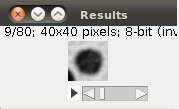
\includegraphics[width=0.75\textwidth]{cropblob.png}  
 % \caption{Difference de Gaussienne (blobs)}
 \end{minipage} \hfill
\begin{minipage}{.450\linewidth}
  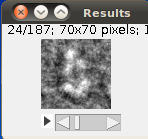
\includegraphics[width=0.5\textwidth]{cropprotDog.png}   
  %\caption{Difference de Gaussienne (protéines)}
 \end{minipage} \hfill
\caption{Exemple d'images formant le stack de particules (blobs et protéines)}
\end{center}
\end{figure}

\subsubsection*{Statistiques}

\begin{itemize}
\item[•] La Différence gaussienne permet d'obtenir les résultats suivants :
\end{itemize}

\begin{figure}[!ht]
\begin{center}
 \begin{minipage}{.450\linewidth}
  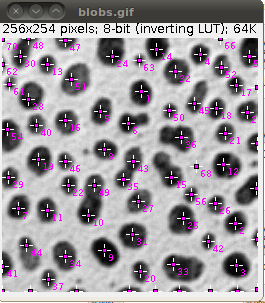
\includegraphics[width=0.75\textwidth]{blobsDog.png}  
 % \caption{Difference de Gaussienne (blobs)}
 \end{minipage} \hfill
\begin{minipage}{.450\linewidth}
  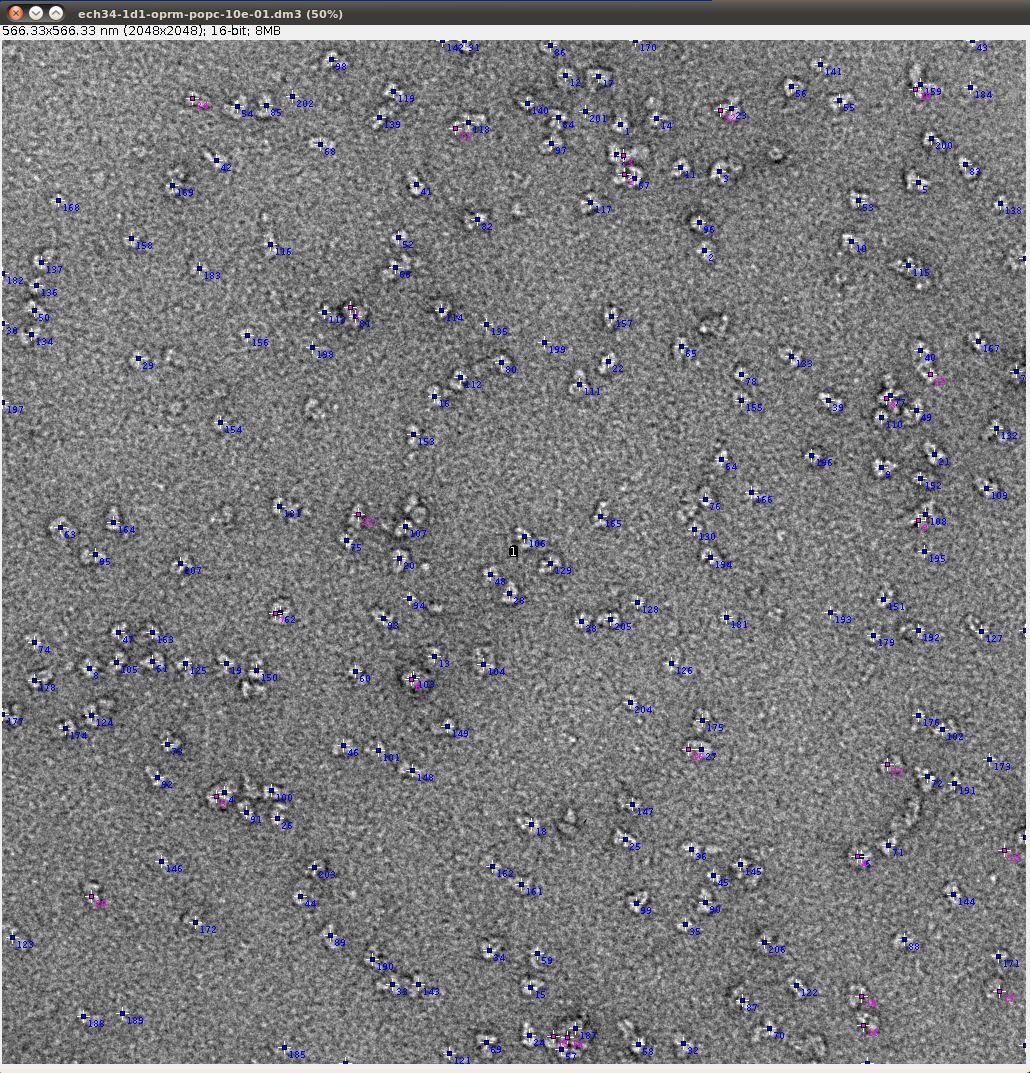
\includegraphics[width=1\textwidth]{protDog.png}   
  %\caption{Difference de Gaussienne (protéines)}
 \end{minipage} \hfill
\caption{Différence Gaussienne (blobs et protéines)}
\end{center}
\end{figure}

Nous constatons que ce piquage est efficace sur notre image de protéines membranaires. Nous l'avons également testé sur une image de blobs, qui est une image de référence pour les essais sur \imj. Cette technique semble tout aussi bien marcher sur les blobs. \\

\begin{itemize}
\item[•] La Différence de dilatation permet d'obtenir les résultats suivants :
\end{itemize}

\begin{figure}[!ht]
\begin{center}
 \begin{minipage}{.450\linewidth}
  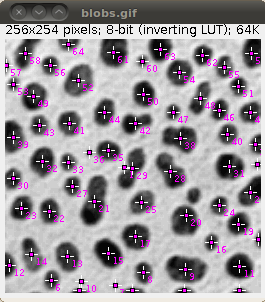
\includegraphics[width=0.75\textwidth]{blobDilate.png}  
 % \caption{Difference de Gaussienne (blobs)}
 \end{minipage} \hfill
\begin{minipage}{.450\linewidth}
  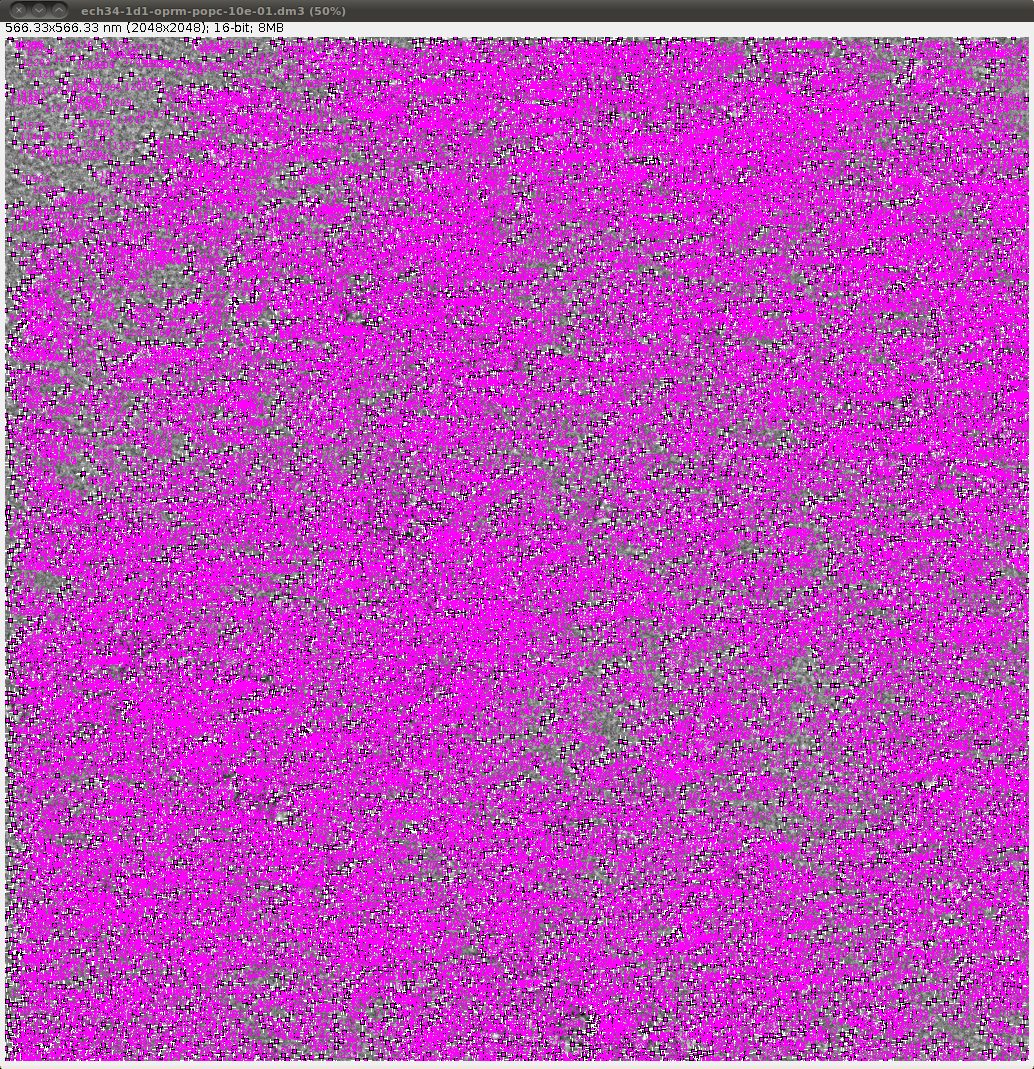
\includegraphics[width=1\textwidth]{protDilate.png}   
  %\caption{Difference de Gaussienne (protéines)}
 \end{minipage} \hfill
\caption{Différence de dilatation (blobs et protéines)}
\end{center}
\end{figure}

Nous observons que cet algorithme semble bien fonctionner sur les blobs, alors que sur les protéines il y a beaucoup trop de points de piquage. Même en modifiant le paramètre de la "Noise Tolerance" nous obtenons des résultats de piquage similaires. \\

\begin{itemize}
\item[•] La Corrélation d'images ne permet pas d'obtenir de résultats de piquage exploitables avec ces deux types d'images. Nous avons également testé cet algorithme avec des images de particules virales. Nous obtenions de bon résultats, cependant, pour des raisons de confidentialité, nous ne pouvons pas intégrer ces images dans notre rapport. \\
\end{itemize}

\begin{itemize}
\item[•] Résultats :
\end{itemize}

Nous avons réalisé une série de tests statistiques afin de comparer l'efficacité de nos algorithmes sur les différentes images. Les résultats obtenus sont regroupés dans le tableau (Table \ref{tableau}) suivant :

\begin{table}[h]
\begin{center}
\begin{tabular}{|c|c|c|c|c|}
\hline
\textbf{Images} & \textbf{Variables} & \textbf{DoG} & \textbf{Dilate Difference} & \textbf{Image Correlation} \\
\hline
Blobs & Vrai Positif (VP) & 63 & 61 & null \\
	& Vrai Négatif (VN) & 3 & 0 & null \\
	& Faux Positif (FP) & 9 & 2 & null \\
	& Faux Négatif (FN) & 0 & 1 & null \\
	& Sensibilité (SE) & 1 & 0.98 & null \\
	& Spécificité (SP) & 0.25 & 0 & null \\
\hline
Protéines & Vrai Positif (VP) & 167 & infini & null \\
	& Vrai Négatif (VN) & 8 & infini & null \\
	& Faux Positif (FP) & 16 & infini & null \\
	& Faux Négatif (FN) & 8 & infini & null \\
	& Sensibilité (SE) & 0.95 & null & null \\
	& Spécificité (SP) & 0.5 & null & null \\
	\hline
\end{tabular}
\end{center}
\caption{Tableau de statistiques d'efficacité des algorithmes de piquage}
\label{tableau}
\end{table}

Les \textbf{Vrais Positifs} sont les particules devant être sélectionnées et qui le sont par l'algorithme. Les \textbf{Vrais Négatifs} représentent tout ce qui ne doit pas être sélectionné et qui ne l'est pas. Les \textbf{Faux Positifs} correspondent à tout ce qui ne doit pas être sélectionné mais qui l'est. Enfin, les \textbf{Faux Négatifs} sont les particules devant être sélectionnées mais qui ne le sont pas. \\ 
Le \textbf{Sensibilité}~\cite{stats:url} est la probabilité qu'une particule devant être piquée le soit. Une mesure de la sensibilité s'accompagne toujours d'une mesure de la spécificité. La \textbf{Spécificité} est la probabilité de ne pas sélectionner ce qui ne doit pas l'être. La sensibilité et la Spécificité sont obtenues par les formules suivantes : \\

\begin{center}
SE = $\frac{\text{VP}}{\text{VP+FN}}$ et SP = $\frac{\text{VN}}{\text{VN+FP}}$ \\
\end{center}

D'après la Table \ref{tableau}, nous remarquons que c'est l'algorithme de Différence gaussienne qui a la meilleure spécificité et sensibilité pour les blobs. En effet, il y a plus de particules sélectionnées avec ce dernier qu'avec la Différence de dilatation, alors que cet algorithme a été créé pour les blobs au départ. Cependant, nous constatons qu'il y a plus de faux positifs avec la Différence gaussienne. \\
En ce qui concerne les protéines, la Différence de dilatation est inefficace car elle ne fait pas de distinction entre le bruit et les particules. La Différence gaussienne, quant à elle, est assez efficace en ce qui concerne la sélection de ces dernières. 

\section{Ajout d'un nouvel algorithme au plugin}

Voici la marche à suivre pour ajouter un nouvel algorithme de piquage à notre plugin :

\begin{itemize}
\item Ajouter le nom de l'algorithme dans la liste des noms proposés par la \emph{JComboBox} dans la classe \texttt{PickFrame}.
\item Ajouter un nouveau "\textit{case}" dans chaque "\textit{switch}" de la classe \texttt{AlgoFactory}.
\item Créer une nouvelle classe \texttt{PanelAlgorithme} dans laquelle doivent se trouver :
	\begin{itemize}
	\item un \emph{JLabel} pour la phrase d'indication d'utilisation de l'algorithme,
	\item tous les \emph{JLabel}, \emph{JCheckBox}, \emph{JButton}, \emph{JTextField}, \emph{JPanel} nécessaires pour le fonctionnement de l'algorithme,
	\item une méthode \texttt{setAttributes()} pour récupérer les paramètres entrés par l'utilisateur,
	\end{itemize}
\item Créer une nouvelle classe \texttt{Algorithme} pour la procédure de piquage suivant le modèle de ceux déjà implantés. 
\end{itemize}




















